\documentclass[a4paper,12pt]{article}
\usepackage[top = 2.5cm, bottom = 2.5cm, left = 2.5cm, right = 2.5cm]{geometry}
\usepackage[T1]{fontenc}
\usepackage[utf8]{inputenc}
\usepackage{multirow} 
\usepackage{booktabs} 
\usepackage{graphicx}
\usepackage[spanish]{babel}
\usepackage{setspace}
\setlength{\parindent}{0in}
\usepackage{float}
\usepackage{fancyhdr}
\usepackage{amsmath}
\usepackage{amssymb}
\usepackage{amsthm}
\usepackage[numbers]{natbib}
\newcommand\Mycite[1]{%
	\citeauthor{#1}~[\citeyear{#1}]}
\usepackage{graphicx}
\usepackage{subcaption}
\usepackage{booktabs}
\usepackage{etoolbox}
\usepackage{minibox}
\usepackage{hyperref}
\usepackage{xcolor}
\usepackage[skins]{tcolorbox}
%---------------------------

\newtcolorbox{cajita}[1][]{
	 #1
}

\newenvironment{sol}
{\renewcommand\qedsymbol{$\square$}\begin{proof}[\textbf{Solución.}]}
	{\end{proof}}

\newenvironment{dem}
{\renewcommand\qedsymbol{$\blacksquare$}\begin{proof}[\textbf{Demostración.}]}
	{\end{proof}}

\newtheorem{problema}{Problema}
\newtheorem{definicion}{Definición}
\newtheorem{ejemplo}{Ejemplo}
\newtheorem{teorema}{Teorema}
\newtheorem{corolario}{Corolario}[teorema]
\newtheorem{lema}[teorema]{Lema}
\newtheorem{prop}{Proposición}
\newtheorem*{nota}{\textbf{NOTA}}
\renewcommand\qedsymbol{$\blacksquare$}
\usepackage{svg}
\usepackage{tikz}
\usepackage[framemethod=default]{mdframed}
\global\mdfdefinestyle{exampledefault}{%
linecolor=lightgray,linewidth=1pt,%
leftmargin=1cm,rightmargin=1cm,
}




\newenvironment{noter}[1]{%
\mdfsetup{%
frametitle={\tikz\node[fill=white,rectangle,inner sep=0pt,outer sep=0pt]{#1};},
frametitleaboveskip=-0.5\ht\strutbox,
frametitlealignment=\raggedright
}%
\begin{mdframed}[style=exampledefault]
}{\end{mdframed}}
\newcommand{\linea}{\noindent\rule{\textwidth}{3pt}}
\newcommand{\linita}{\noindent\rule{\textwidth}{1pt}}

\AtBeginEnvironment{align}{\setcounter{equation}{0}}
\pagestyle{fancy}

\fancyhf{}









%----------------------------------------------------------
\lhead{\footnotesize Álgebra Moderna}
\rhead{\footnotesize  Rudik Roberto Rompich}
\cfoot{\footnotesize \thepage}


%--------------------------

\begin{document}
 \thispagestyle{empty} 
    \begin{tabular}{p{15.5cm}}
    \begin{tabbing}
    \textbf{Universidad del Valle de Guatemala} \\
    Departamento de Matemática\\
    Licenciatura en Matemática Aplicada\\\\
   \textbf{Estudiante:} Rudik Roberto Rompich\\
   \textbf{Correo:}  \href{mailto:rom19857@uvg.edu.gt}{rom19857@uvg.edu.gt}\\
   \textbf{Carné:} 19857
    \end{tabbing}
    \begin{center}
        MM2035 - Álgebra Moderna - Catedrático: Ricardo Barrientos\\
        \today
    \end{center}\\
    \hline
    \\
    \end{tabular} 
    \vspace*{0.3cm} 
    \begin{center} 
    {\Large \bf  Tarea 13
} 
        \vspace{2mm}
    \end{center}
    \vspace{0.4cm}
%--------------------------

\begin{problema}
    Usted está realizando un experimento de efecto fotoeléctrico mediante luz de 500 de longitud de onda a un trozo de metal y determinar el potencial de parada. Si, sin saberlo de que su fuente de luz de 500 nm contiene en realidad una pequeña cantidad de luz ultravioleta, ¿se alterarían los resultados los resultados en una pequeña cantidad o en una gran cantidad? Explícalo.
    \begin{sol}
        Los resultados se alterarían en una gran cantidad. Esto incluso lo comprobamos en un laboratorio que tuvimos en clase. Esto se debe a que la luz ultravioleta logrará sobrepasar la barrera electroestática del trozo metal. 
    \end{sol}
\end{problema}


\begin{problema}

    Un átomo aislado puede emitir un fotón, y la energía interna del átomo disminuye. De hecho, el proceso tiene un nombre: emisión espontánea. ¿Puede un electrón aislado emitir un fotón? ¿Por qué sí o por qué no?
    \begin{sol}
        No, no puede. El electrón y el fotón son partículas elementales, una no puede emitir a la otra. 
    \end{sol}
    
    \end{problema}
    
    
    \begin{problema}
        Un haz de luz coherente incide en una sola rendija y produce un patrón de difracción extendido más allá. El número de fotones detectados por unidad de tiempo en un detector en el centro del patrón es $X$. Ahora se abren otras dos rendijas cercanas, de la misma anchura que la original, igualmente espaciadas a ambos lados de la misma, e igualmente bien que se comporta como partículas iluminado por el haz. ¿Cuántos fotones serán detectados por unidad de tiempo en el detector central ahora? ¿Por qué?
        \begin{sol}
            Serán $9X$, porque el campo eléctrico producido es 3 veces más grande de lo que originalmente era y por lo tanto también 3 fotones se están detectando por cada uno. 
        \end{sol}
    
    \end{problema}
    
    
    \begin{problema}
        ¿A qué longitud de onda emite el cuerpo humano la máxima radiación electromagnética? Utilice la ley de Wien y suponga una temperatura de la piel de $70^{\circ} \mathrm{F}$.
        \begin{sol}
            Tenemos:
            \begin{align*}
                \lambda_ {\max} T & = 2.898x10^{-3}m\cdot K \\
                \lambda_{\max} (70^{\circ} \mathrm{F})&= 2.898x10^{-3}m\cdot K \\
                \lambda_{\max} [(70^{\circ} \mathrm{F}-32)\cdot 5/9 + 273.15]&= 2.898x10^{-3}m\cdot K \\
                \lambda_{\max} &= \frac{2.898x10^{-3}m\cdot K }{294.261K}\\
                &= 9.85x10^{-6}m
            \end{align*}
            Por lo tanto, la longitud de onda está en el infrarrojo. 
        \end{sol}
    \end{problema}
    
    
    \begin{problema}
    
    Usted es un físico experimental de principios del siglo $X X$ y no conoce el valor de la constante de Planck. Mediante un gráfico adecuado de los siguientes datos, y utilizando la explicación de Einstein para el efecto fotoeléctrico ($K E=h f-\phi$, donde h no se conoce), determine la constante de Planck.
    \begin{center}
        \begin{tabular}{cc}
            Wavelength of Light $(\mathbf{n m})$ & Stopping Potential $(\mathbf{V})$ \\
            \hline 550 & $0.060$ \\
            \hline 500 & $0.286$ \\
            \hline 450 & $0.563$ \\
            \hline 400 & $0.908$ \\
            \hline
            \end{tabular}
    \end{center}
    
    \begin{sol}
        Tenemos 
        \begin{align*}
            K E&=h f-\phi\\
            eV_{\text{stop}}&= h\cdot \frac{c}{\lambda}-\phi
        \end{align*}
        Ya que tenemos $V$ y $1/\lambda$, esta ecuación se convierte en
         $$V_{\text{stop}}= h\cdot \frac{c}{e}$$
         Tal que graficando los datos tenemos: 
         \begin{figure}[H]
            \centering
            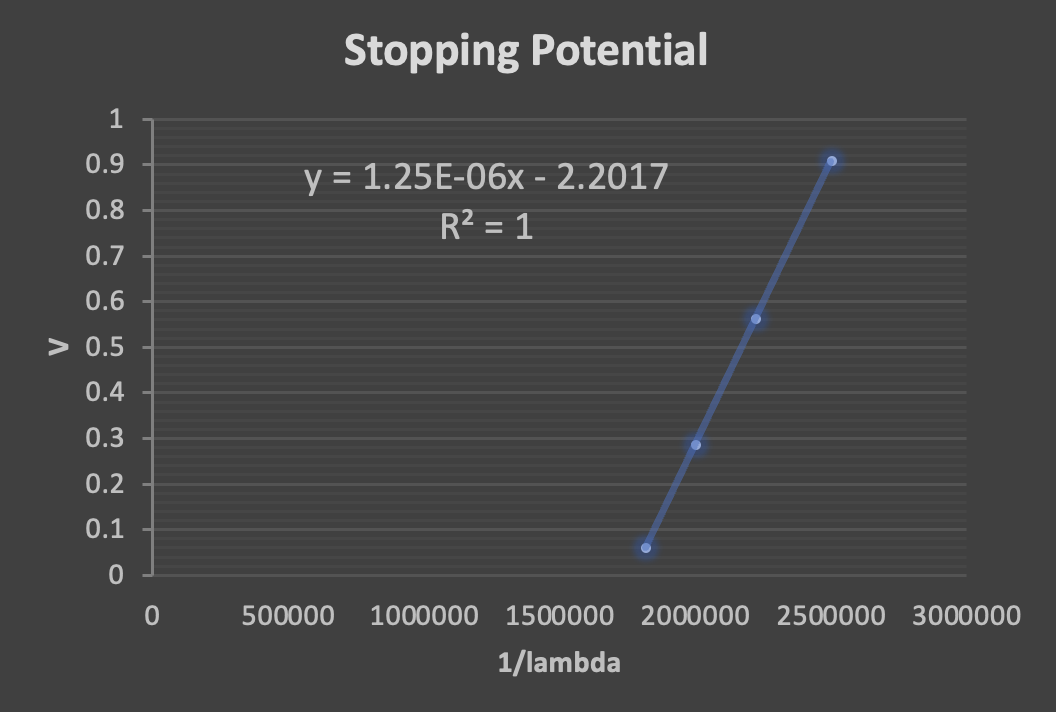
\includegraphics[scale=0.5]{imagenes/1.png}
         \end{figure}
        Entonces la relación se convierte en 
        $$1.25x10^{-6} V\cdot m= h\cdot \frac{3x10^8 m/s}{1.603 x10^{-19}C}$$
        Al despejar para $h$, entonces la constante de Plank es: 
        $$h=6.67x10^{-34}J\cdot s$$
    \end{sol}
    \end{problema}
    
    
    \begin{problema}
    Cuando un haz de electrones monoenergéticos se dirige a un blanco de tungsteno, se producen rayos $X$ con longitudes de onda no inferiores a 0,062 $\mathrm{nm}$. ¿A qué velocidad se mueven los electrones en el haz se mueven?
    \begin{sol}
        Tenemos:
        \begin{align*}
            KE_{\text{electrón}} &= hf-\phi\\
            \frac{1}{2}mv^2 &= h\cdot \frac{c}{\lambda}-\phi\\
            \frac{1}{2}mv^2 &= h\cdot \frac{c}{\lambda}\\
            v &=\pm \sqrt{h\cdot \frac{2c}{\lambda}}\\
            v &=\pm \sqrt{(6.63x10{-34} J\cdot s)\cdot \frac{2\cdot (3x10^8 m/s)}{0.062x10^{-9}m}}\\
            v &= 8.15 x 10^{7}m/s
        \end{align*}
    \end{sol}
    
    \end{problema}
    
    
    \begin{problema}
        Un fotón se dispersa en un electrón libre. 
        $$\Delta \lambda = \frac{h}{mc}(1-\cos \theta)$$
        \begin{enumerate}
            \item (a) ¿Cuál es el máximo cambio posible en la longitud de onda?
            \begin{sol}
                Tenemos, 
                \begin{align*}
                    \Delta \lambda &= \frac{h}{mc}\cdot 2\\
                                   &= \frac{6.63x10^{-34}J\cdot s}{(9.11x10^{-31}kg)(3x10^8 m/s)}\cdot 2\\
                                   &= 0.00485 x10^{-9}m
                \end{align*}
            \end{sol} 
            \item (b) Suponga que un fotón se dispersa en un protón libre. ¿Cuál es el máximo cambio posible en la longitud de onda?
            \begin{sol}
                Tenemos, 
                \begin{align*}
                    \Delta \lambda &= \frac{h}{mc}\cdot 2\\
                                   &= \frac{6.63x10^{-34}J\cdot s}{(1.67x10^{-27}kg)(3x10^8 m/s)}\cdot 2\\
                                   &= 0.00000265x10^{-9}m
                \end{align*}
            \end{sol} 
            \item (c) ¿Qué demuestra más claramente la naturaleza de partícula de la radiación electromagnética: la colisión con un electrón o la colisión con un protón?
            \begin{sol}
                La colisión de un electrón, es mucho más grande que la de un protón. 
            \end{sol}
        \end{enumerate}        
        
    \end{problema}
    
    
    \begin{problema}
        En la tomografía por emisión de positrones (PET), un electrón y un positrón se aniquilan, y se detectan dos fotones de una energía característica. ¿Cuál es esta energía? y ¿cuál es la longitud de onda correspondiente? Se puede suponer que el para es esencialmente estacionario antes de la aniquilación.
        \begin{sol}
            \begin{itemize}
                \item La energía es: 
                \begin{align*}
                    E &= 2\left[\frac{1}{2}mv^2\right]\\
                      &= mv^2\\
                      &= (9.11x10^{-31} kg)(3x10^8 m/s)^2\\
                      &= 8.2 x 10^{-14}J
                \end{align*}
                \item Longitud de onda: 
                \begin{align*}
                    KE &= hf\\
                    KE &= \frac{ h\cdot c}{\lambda}
                    \intertext{Despejando para $\lambda$:}
                    \lambda &= \frac{(6.63x10^{-34} J\cdot s)(3x10^8 m/s)}{8.2 x 10^{-14}J}\\
                    &=  2.42 x 10^{-12}m
                \end{align*}
            \end{itemize}
        \end{sol}
    \end{problema}
    
    
    \begin{problema}
        Las ondas electromagnéticas inciden en una única rendija de $1 \mu \mathrm{m}$ de anchura. Determine la anchura total angular (ángulo desde primer mínimo a un lado del centro al primer mínimo en el otro) en grados del máximo de difracción central si las ondas son 
        \begin{cajita}
            \begin{enumerate}
                \item Primer mínimo 
                \begin{align*}
                    a\sin\theta &= \lambda\\
                    \theta &= \sin^{-1}\left(\frac{\lambda}{a}\right)
                \end{align*}
                \item Mínimo del otro lado 
                \begin{align*}
                    \Delta\theta &= 2\sin^{-1}\left(\frac{\lambda}{a}\right)
                \end{align*}
            \end{enumerate}
            
        \end{cajita}
        \begin{enumerate}
            \item (a) luz visible de longitud de onda $500$ nm 
            \begin{sol}
                Tenemos, 
                \begin{align*}
                    \Delta\theta &= 2\sin^{-1}\left(\frac{\lambda}{a}\right)\\
                    &= 2\sin^{-1}\left(\frac{500x10^{-9}m}{1x10^{-6}m}\right)\\
                    &= 60^{\circ}
                \end{align*}
            \end{sol}
            \item (b) rayos $X$ de longitud de onda 0,05 $\mathrm{nm}$.
            \begin{sol}
                Tenemos, 
                \begin{align*}
                    \Delta\theta &= 2\sin^{-1}\left(\frac{\lambda}{a}\right)\\
                    &= 2\sin^{-1}\left(\frac{0.05x10^{-9}m}{1x10^{-6}m}\right)\\
                    &= 5.73x10^{-3\circ}
                \end{align*}
            \end{sol}
            \item (c) ¿Cuál de ellas demuestra más claramente la naturaleza ondulatoria?
            \begin{sol}
                La luz visible, es mucho más grande que los rayos X. 
            \end{sol}
        \end{enumerate}
        
        
    \end{problema}
    
    
    \begin{problema}
        Un electrón que se mueve hacia la izquierda a 0,8c colisiona con un fotón entrante que se mueve hacia la derecha. Después de la colisión el electrón se mueve hacia la derecha a 0,6c y un fotón saliente se mueve hacia la izquierda. ¿Cuál era la longitud de onda del fotón entrante?
        \begin{sol}
            Tenemos los siguientes datos:
            \begin{enumerate}
                \item Inicio: 
                \begin{enumerate}
                    \item Electrón hacia la izquierda a $0.8c$
                    \item Protón hacia la derecha
                \end{enumerate}
                \item Final: 
                \begin{enumerate}
                    \item Electrón hacia la derecha a $0.6c$
                    \item Protón hacia la izquierda.
                \end{enumerate}
                Además, tenemos las siguientes ecuaciones:
                \begin{enumerate}
                    \item Conservación del momento
                    $$\frac{h}{\lambda}-\gamma_i m_eu_i= \gamma_f m_e u_f -\frac{h}{\lambda'}$$
                    \item Conservación de la energía 
                    $$\frac{hc}{\lambda}+\gamma_i m_ec^2 = \gamma_f m_e c^2 +\frac{hc}{\lambda'}$$
                \end{enumerate}
                Ahora bien, de la conservación del momento, tenemos:
                \begin{align*}
                    \frac{h}{\lambda'} &=  \gamma_i m_eu_i  +\gamma_f m_e u_f -\frac{h}{\lambda}
                    \intertext{Multiplicando por $c$:}
                    \frac{hc}{\lambda'} &=  c\gamma_i m_eu_i  +c\gamma_f m_e u_f -\frac{hc}{\lambda}
                    \intertext{Sustituyendo en la ecuación de la conservación de la energía: }
                    \frac{hc}{\lambda}+\gamma_i m_ec^2 &= \gamma_f m_e c^2 +c\gamma_i m_eu_i  +c\gamma_f m_e u_f -\frac{hc}{\lambda}\\
                    \frac{2hc}{\lambda} &= \gamma_f m_e c^2 +c\gamma_i m_eu_i  +c\gamma_f m_e u_f -\gamma_i m_ec^2
                \end{align*} 
                De esto, obtemos: 
                \begin{align*}
                    \lambda &= \frac{2hc}{\gamma_f m_e c^2 +c\gamma_i m_eu_i  +c\gamma_f m_e u_f -\gamma_i m_ec^2}\\
                    &= \frac{2hc}{(\gamma_f-\gamma_i) m_e c^2 +c\gamma_i m_eu_i  +c\gamma_f m_e u_f}
                    \intertext{En donde, $u_i=0.8c,u_f=0.6c,\gamma_i=1.62,\gamma_f=1.25$.}
                \end{align*}
                Con lo cual, obtenemos: 
                $$\lambda = 2.91x10^{-12}m$$
            \end{enumerate}
        \end{sol}
    \end{problema}
    
    
    





%---------------------------
%\bibliographystyle{apa}
%\bibliography{referencias.bib}

\end{document}